\documentclass{standalone}
\usepackage{tikz}
\usetikzlibrary{patterns, positioning}

\begin{document}
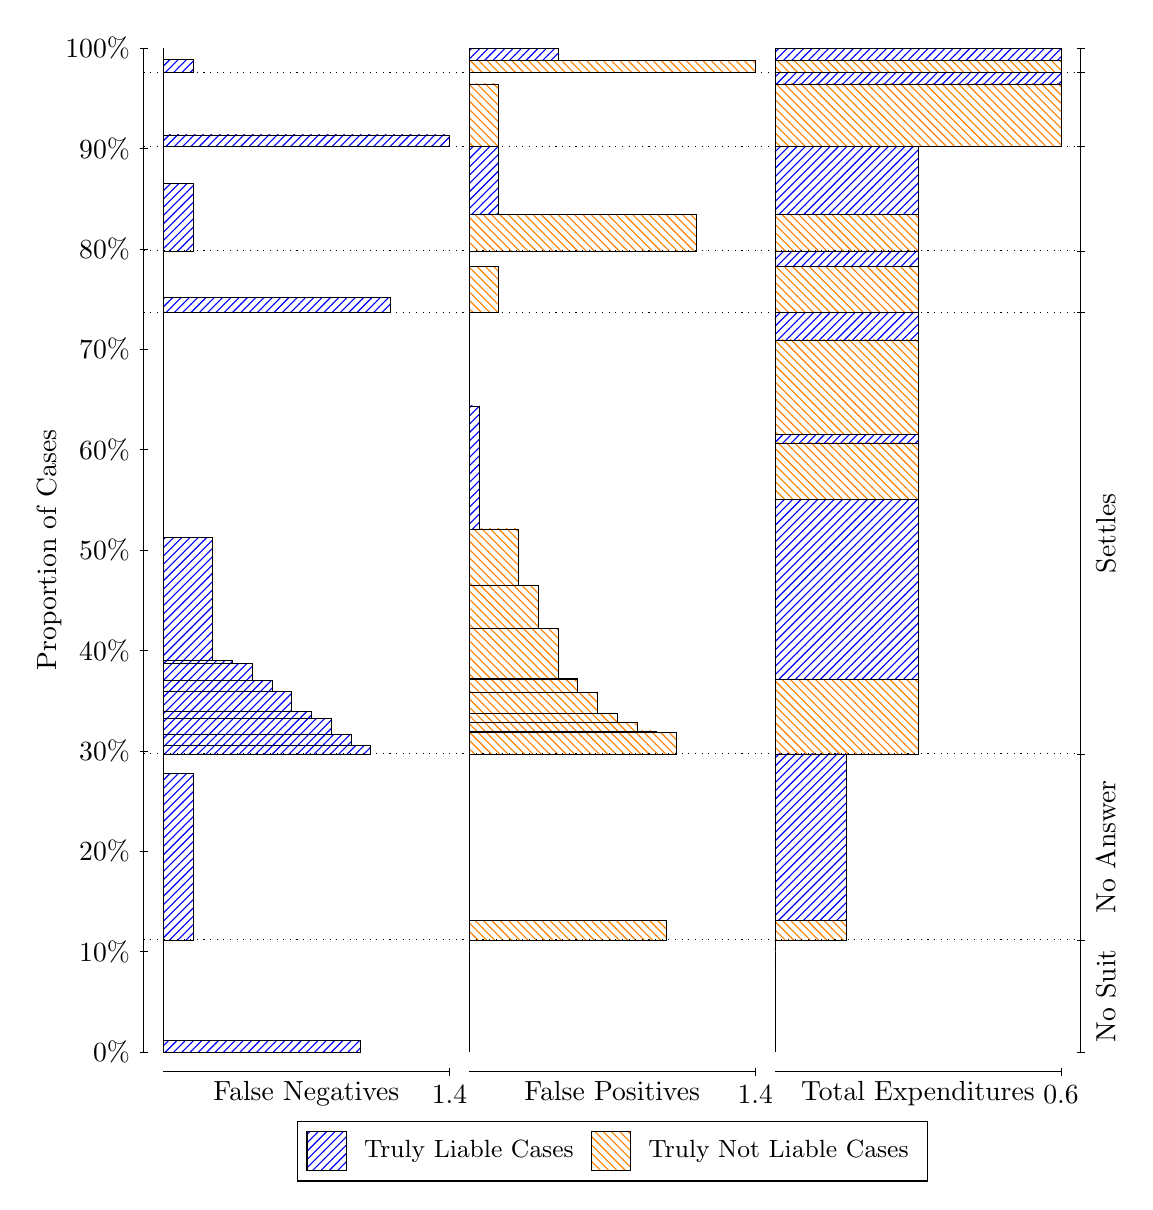
\begin{tikzpicture}
\draw[black, very thin] (1.5,1.75) -- (1.5,14.5);
\node[rotate=90, anchor=center] at (0.3, 8.125) {Proportion of Cases};
\draw[black, very thin] (1.45,1.75) -- (1.55,1.75);
\node[anchor=east] at (1.45, 1.75) {0\%};
\draw[black, very thin] (1.45,3.025) -- (1.55,3.025);
\node[anchor=east] at (1.45, 3.025) {10\%};
\draw[black, very thin] (1.45,4.3) -- (1.55,4.3);
\node[anchor=east] at (1.45, 4.3) {20\%};
\draw[black, very thin] (1.45,5.575) -- (1.55,5.575);
\node[anchor=east] at (1.45, 5.575) {30\%};
\draw[black, very thin] (1.45,6.85) -- (1.55,6.85);
\node[anchor=east] at (1.45, 6.85) {40\%};
\draw[black, very thin] (1.45,8.125) -- (1.55,8.125);
\node[anchor=east] at (1.45, 8.125) {50\%};
\draw[black, very thin] (1.45,9.4) -- (1.55,9.4);
\node[anchor=east] at (1.45, 9.4) {60\%};
\draw[black, very thin] (1.45,10.675) -- (1.55,10.675);
\node[anchor=east] at (1.45, 10.675) {70\%};
\draw[black, very thin] (1.45,11.95) -- (1.55,11.95);
\node[anchor=east] at (1.45, 11.95) {80\%};
\draw[black, very thin] (1.45,13.225) -- (1.55,13.225);
\node[anchor=east] at (1.45, 13.225) {90\%};
\draw[black, very thin] (1.45,14.5) -- (1.55,14.5);
\node[anchor=east] at (1.45, 14.5) {100\%};

\draw[black, very thin] (13.4,1.75) -- (13.4,14.5);
\draw[black, very thin] (13.35,1.75) -- (13.45,1.75);
\node[anchor=west] at (13.35, 1.75) {};
\draw[black, very thin] (13.35,3.1734) -- (13.45,3.1734);
\node[anchor=west] at (13.35, 3.1734) {};
\draw[black, very thin] (13.35,5.5354) -- (13.45,5.5354);
\node[anchor=west] at (13.35, 5.5354) {};
\draw[black, very thin] (13.35,11.139) -- (13.45,11.139);
\node[anchor=west] at (13.35, 11.139) {};
\draw[black, very thin] (13.35,11.925) -- (13.45,11.925);
\node[anchor=west] at (13.35, 11.925) {};
\draw[black, very thin] (13.35,13.247) -- (13.45,13.247);
\node[anchor=west] at (13.35, 13.247) {};
\draw[black, very thin] (13.35,14.193) -- (13.45,14.193);
\node[anchor=west] at (13.35, 14.193) {};
\draw[black, very thin] (13.35,14.5) -- (13.45,14.5);
\node[anchor=west] at (13.35, 14.5) {};

\draw[black, very thin, pattern color=blue, pattern=north east lines] (1.75,1.75) rectangle (4.2557,1.8998);
\draw[black, very thin, pattern color=orange, pattern=north west lines] (1.75,1.8998) rectangle (1.75,3.1734);
\draw[black, very thin, pattern color=blue, pattern=north east lines] (1.75,3.1734) rectangle (2.1259,5.2909);
\draw[black, very thin, pattern color=orange, pattern=north west lines] (1.75,5.2909) rectangle (1.75,5.5354);
\draw[black, very thin, pattern color=blue, pattern=north east lines] (1.75,5.5354) rectangle (4.381,5.6475);
\draw[black, very thin, pattern color=blue, pattern=north east lines] (1.75,5.6475) rectangle (4.1305,5.7798);
\draw[black, very thin, pattern color=blue, pattern=north east lines] (1.75,5.7798) rectangle (3.8799,5.9893);
\draw[black, very thin, pattern color=blue, pattern=north east lines] (1.75,5.9893) rectangle (3.6293,6.0797);
\draw[black, very thin, pattern color=blue, pattern=north east lines] (1.75,6.0797) rectangle (3.3787,6.329);
\draw[black, very thin, pattern color=blue, pattern=north east lines] (1.75,6.329) rectangle (3.1282,6.4662);
\draw[black, very thin, pattern color=blue, pattern=north east lines] (1.75,6.4662) rectangle (2.8776,6.6803);
\draw[black, very thin, pattern color=blue, pattern=north east lines] (1.75,6.6803) rectangle (2.627,6.7193);
\draw[black, very thin, pattern color=blue, pattern=north east lines] (1.75,6.7193) rectangle (2.3764,8.2806);
\draw[black, very thin, pattern color=orange, pattern=north west lines] (1.75,8.2806) rectangle (1.75,11.139);
\draw[black, very thin, pattern color=blue, pattern=north east lines] (1.75,11.139) rectangle (4.6316,11.333);
\draw[black, very thin, pattern color=orange, pattern=north west lines] (1.75,11.333) rectangle (1.75,11.925);
\draw[black, very thin, pattern color=blue, pattern=north east lines] (1.75,11.925) rectangle (2.1259,12.783);
\draw[black, very thin, pattern color=orange, pattern=north west lines] (1.75,12.783) rectangle (1.75,13.247);
\draw[black, very thin, pattern color=blue, pattern=north east lines] (1.75,13.247) rectangle (5.3833,13.396);
\draw[black, very thin, pattern color=orange, pattern=north west lines] (1.75,13.396) rectangle (1.75,14.193);
\draw[black, very thin, pattern color=blue, pattern=north east lines] (1.75,14.193) rectangle (2.1259,14.354);
\draw[black, very thin, pattern color=orange, pattern=north west lines] (1.75,14.354) rectangle (1.75,14.5);
\draw[black, very thin, pattern color=orange, pattern=north west lines] (5.6333,1.75) rectangle (5.6333,3.0237);
\draw[black, very thin, pattern color=blue, pattern=north east lines] (5.6333,3.0237) rectangle (5.6333,3.1734);
\draw[black, very thin, pattern color=orange, pattern=north west lines] (5.6333,3.1734) rectangle (8.1391,3.4179);
\draw[black, very thin, pattern color=blue, pattern=north east lines] (5.6333,3.4179) rectangle (5.6333,5.5354);
\draw[black, very thin, pattern color=orange, pattern=north west lines] (5.6333,5.5354) rectangle (8.2644,5.8057);
\draw[black, very thin, pattern color=orange, pattern=north west lines] (5.6333,5.8057) rectangle (8.0138,5.8286);
\draw[black, very thin, pattern color=orange, pattern=north west lines] (5.6333,5.8286) rectangle (7.7632,5.937);
\draw[black, very thin, pattern color=orange, pattern=north west lines] (5.6333,5.937) rectangle (7.5126,6.051);
\draw[black, very thin, pattern color=orange, pattern=north west lines] (5.6333,6.051) rectangle (7.2621,6.318);
\draw[black, very thin, pattern color=orange, pattern=north west lines] (5.6333,6.318) rectangle (7.0115,6.4811);
\draw[black, very thin, pattern color=orange, pattern=north west lines] (5.6333,6.4811) rectangle (7.0115,6.4979);
\draw[black, very thin, pattern color=orange, pattern=north west lines] (5.6333,6.4979) rectangle (6.7609,7.1325);
\draw[black, very thin, pattern color=orange, pattern=north west lines] (5.6333,7.1325) rectangle (6.5103,7.6774);
\draw[black, very thin, pattern color=orange, pattern=north west lines] (5.6333,7.6774) rectangle (6.2598,8.3934);
\draw[black, very thin, pattern color=blue, pattern=north east lines] (5.6333,8.3934) rectangle (5.7586,9.9547);
\draw[black, very thin, pattern color=blue, pattern=north east lines] (5.6333,9.9547) rectangle (5.6333,11.139);
\draw[black, very thin, pattern color=orange, pattern=north west lines] (5.6333,11.139) rectangle (6.0092,11.731);
\draw[black, very thin, pattern color=blue, pattern=north east lines] (5.6333,11.731) rectangle (5.6333,11.925);
\draw[black, very thin, pattern color=orange, pattern=north west lines] (5.6333,11.925) rectangle (8.5149,12.389);
\draw[black, very thin, pattern color=blue, pattern=north east lines] (5.6333,12.389) rectangle (6.0092,13.247);
\draw[black, very thin, pattern color=orange, pattern=north west lines] (5.6333,13.247) rectangle (6.0092,14.044);
\draw[black, very thin, pattern color=blue, pattern=north east lines] (5.6333,14.044) rectangle (5.6333,14.193);
\draw[black, very thin, pattern color=orange, pattern=north west lines] (5.6333,14.193) rectangle (9.2667,14.34);
\draw[black, very thin, pattern color=blue, pattern=north east lines] (5.6333,14.34) rectangle (6.7609,14.5);
\draw[black, very thin, pattern color=orange, pattern=north west lines] (9.5167,1.75) rectangle (9.5167,3.0237);
\draw[black, very thin, pattern color=blue, pattern=north east lines] (9.5167,3.0237) rectangle (9.5167,3.1734);
\draw[black, very thin, pattern color=orange, pattern=north west lines] (9.5167,3.1734) rectangle (10.425,3.4179);
\draw[black, very thin, pattern color=blue, pattern=north east lines] (9.5167,3.4179) rectangle (10.425,5.5354);
\draw[black, very thin, pattern color=orange, pattern=north west lines] (9.5167,5.5354) rectangle (11.333,6.4811);
\draw[black, very thin, pattern color=blue, pattern=north east lines] (9.5167,6.4811) rectangle (11.333,8.7687);
\draw[black, very thin, pattern color=orange, pattern=north west lines] (9.5167,8.7687) rectangle (11.333,9.4847);
\draw[black, very thin, pattern color=blue, pattern=north east lines] (9.5167,9.4847) rectangle (11.333,9.5968);
\draw[black, very thin, pattern color=orange, pattern=north west lines] (9.5167,9.5968) rectangle (11.333,10.793);
\draw[black, very thin, pattern color=blue, pattern=north east lines] (9.5167,10.793) rectangle (11.333,11.139);
\draw[black, very thin, pattern color=orange, pattern=north west lines] (9.5167,11.139) rectangle (11.333,11.731);
\draw[black, very thin, pattern color=blue, pattern=north east lines] (9.5167,11.731) rectangle (11.333,11.925);
\draw[black, very thin, pattern color=orange, pattern=north west lines] (9.5167,11.925) rectangle (11.333,12.389);
\draw[black, very thin, pattern color=blue, pattern=north east lines] (9.5167,12.389) rectangle (11.333,13.247);
\draw[black, very thin, pattern color=orange, pattern=north west lines] (9.5167,13.247) rectangle (13.15,14.044);
\draw[black, very thin, pattern color=blue, pattern=north east lines] (9.5167,14.044) rectangle (13.15,14.193);
\draw[black, very thin, pattern color=orange, pattern=north west lines] (9.5167,14.193) rectangle (13.15,14.34);
\draw[black, very thin, pattern color=blue, pattern=north east lines] (9.5167,14.34) rectangle (13.15,14.5);
\draw[black, dotted] (1.5,3.1734) -- (13.4,3.1734);
\draw[black, dotted] (1.5,5.5354) -- (13.4,5.5354);
\draw[black, dotted] (1.5,11.139) -- (13.4,11.139);
\draw[black, dotted] (1.5,11.925) -- (13.4,11.925);
\draw[black, dotted] (1.5,13.247) -- (13.4,13.247);
\draw[black, dotted] (1.5,14.193) -- (13.4,14.193);
\draw[black, very thin] (1.75,1.5) -- (5.3833,1.5);
\node[anchor=north] at (3.5667, 1.5) {False Negatives};
\draw[black, very thin] (5.3833,1.45) -- (5.3833,1.55);
\node[anchor=north] at (5.3833, 1.45) {1.4};

\draw[black, very thin] (5.6333,1.5) -- (9.2667,1.5);
\node[anchor=north] at (7.45, 1.5) {False Positives};
\draw[black, very thin] (9.2667,1.45) -- (9.2667,1.55);
\node[anchor=north] at (9.2667, 1.45) {1.4};

\draw[black, very thin] (9.5167,1.5) -- (13.15,1.5);
\node[anchor=north] at (11.333, 1.5) {Total Expenditures};
\draw[black, very thin] (13.15,1.45) -- (13.15,1.55);
\node[anchor=north] at (13.15, 1.45) {0.6};

\node[black, centered, rotate=90] at (13.72, 2.4617) {No Suit};
\node[black, centered, rotate=90] at (13.72, 4.3544) {No Answer};
\node[black, centered, rotate=90] at (13.72, 8.337) {Settles};





\draw (7.449999999999999,1.5) node[draw=none] (baseCoordinate) {};
\begin{scope}[align=center]
        \matrix[scale=0.5, draw=black, below=0.5cm of baseCoordinate, nodes={draw}, column sep=0.1cm]{
            \node[rectangle, draw, minimum width=0.5cm, minimum height=0.5cm, pattern=north east lines, pattern color=blue] {}; &
            \node[draw=none, font=\small] (B) {Truly Liable Cases}; &
            \node[rectangle, draw, minimum width=0.5cm, minimum height=0.5cm, pattern=north west lines, pattern color=orange] {}; &
            \node[draw=none, font=\small] (B) {Truly Not Liable Cases}; \\
            };
\end{scope}

\end{tikzpicture}
\end{document}